\documentclass[main]{subfiles}
\usepackage{tikz}

\begin{document}
%Set chapter counter as week-1
\chapPreamble{9}{March 31, 2023}{Random walk in trap environment}
%Set chapter name

\lecture{Siva Athreya}{Sanchayan Bhowal, Ramkrishna Samanta}

\section{Continuous time random walk}
In this model the random walker wasits an exponential amount of time to perform a jump like a discrete time random walk. Consider $\{V_i : i\geq 1\}$ to be a collection of independent Exponential$(\lambda)$ random variables. Let $\lambda=1$. Define $T_k$ to be the sum of the first $k$ $V_i$'s. Also, define $N_t$ to be the number of $T_k$ less than $t$. Hence,
\begin{itemize}
    \item $\P(V_i \leq t)=1-e^{-t}$
    \item $T_k=\sum_{i=1}^{k}V_i$
    \item $N_t=\sum_{k=1}^{\infty}\one(T_k\leq t)$
    \item $\{N_t=k\}=\{T_k\leq T_{k+1}\}$
\end{itemize}
\begin{theorem}
    \begin{enumerate}
        \item $N_t\sim$ Poisson$(t)$
        \item $N_t-N_s$ is independent of $N_r$ where $r\leq s \leq t$.
        \item For $0\leq t_0 \leq t_1 \leq \ldots \leq t_n$
              $$
                  \{N_{t_{i+1}}-N_{t_i}: i=0,\ldots, n-1\} \text{ are independent}
              $$
              So, $N_{t_{i+1}}-N_{t_i}\sim$ Poisson$(t_{i+1}-t_i)$
    \end{enumerate}
\end{theorem}
\begin{definition}
    Let $U_n: n\geq 0$ be a random walk on $(\Gamma,\mu)$. Define, a continuous time random walk on $(\Gamma,\mu)$ with rate 1 to be:
    $$Y_t=U_{N_t} \hfill \forall t\geq 0$$.
\end{definition}
\begin{remark}
    The random variable $Y_t$ is a random step function which is right continuous with left limits.
\end{remark}

\section{Random walk in trap environment}
\subsection*{Continuous Time set-up}
Consider the graph $\Z^d$ with natural weights. Let $\{X_t\}_{t\geq 0}$ be a continuous time random walk on $\Z^d$ starting at 0, with rate $\kappa$. Now, let us set up the traps, i.e., for each $y\in \Z^d$ let $N_y\sim$Poisson$(\rho)$. This $N_y$ denote the number of \textit{traps} at $y$. Each trap($Y^{j,y}$) perform a continuous time random walk$(\{Y^{j,y}_t\}_{t\geq 0})$ with rate $\nu$; where $1\leq j \leq N_y$. The random walk gets killed if it meets a trap. There are two ways of killing viz,
\begin{itemize}
    \item [Hard] The walk gets killed upon intersection with any $Y^{j,y}$.
    \item [Soft] At each site $x$ at time $t\geq 0$, define
          $$
              \xi(t,x):=\sum_{y \in \Z^d,1\leq j \leq N_y} \# \{Y^{j,y}\text{ at }x\}.
          $$
          Now $X_t$ gets killed at rate $\gamma\xi(t,x)$ where $\gamma \in \R$.
\end{itemize}
\begin{remark}
    Hard killing infact corresponds to $\gamma=\infty$ case of soft killing.
\end{remark}
The probability of survival is given by
\begin{equation*}
    Z_{\gamma,t}=\E^X[\exp(-\gamma\int_{0}^{t}\xi(s,X(s))ds)]
\end{equation*}
\subsection*{Discrete Time set-up}
Let $\{X_t\}_{t\geq 0}$ be a random walk on $\Z^d$ with natural weights starting at 0. For each $y\in \Z^d$ let $N_y\sim$Poisson$(\rho)$ denotes the number of traps at $y$. Each trap($Y^{j,y}$) perform a lazy random walk$(\{Y^{j,y}_t\}_{t\geq 0})$ on $\Z^d$; where $1\leq j \leq N_y$. The trap kills the random walk with probability $q$ if it meets the random walk; $q \in (0,1)$.
Let $\xi(n,x)$ denote the number of traps at location $x$, i.e.
$$
    \xi(n,x)=\sum_{y \in \Z^d,1\leq j \leq N_y} \delta_x(Y^{j,y}_n).
$$
Assume $X_k$ has survived till $k\leq n$. Given $X_n$ the probability that $X_n$ will survive at time $n$ is $(1-q)^{\xi(n,X_n)}$.
Hence,
\begin{equation}
    \begin{aligned}
        \sigma^X(n,\xi) & =\P(X\text{ has survived till time } n \text{ given } \{Y^{j,y}_m\}_{1\leq j \leq m, y \in \Z^d} \text{ where } m\leq n) \\
                        & =(1-q)^{\sum_{i=1}^{n}\xi(i,X_i)}.
    \end{aligned}
\end{equation}
\section{Pascal's Theorem}
The average survival probability of a given trajectory $X$ is given by $\sigma^X(n)=\E^\xi[(1-q)^{\sum_{i=1}^{n}\xi(i,X_i)}]$.
\begin{theorem}[Pascal]
    The survival probability is maximized by the trajectory $\zero$ where $\zero_k=0$ for every $k \in \N\cup{0}$, i.e,
    $$\sigma^X(n)\leq \sigma^\zero(n).$$
\end{theorem}
\begin{lemma}
    $\sigma^X(n)=\exp (-\lambda \sum_{y \in \Z^d}W_X(n,y))$ where $W_X(n,y)=1-\E^y[1-(1-q)^{\sum_{i=1}^{n}\delta(Y_i^y)}]$. The $Y_i^y$ is a random variable with ditribution same as i.i.d. $Y_i^{j,y}$.
\end{lemma}
\begin{proof}
    Let $X:\N\cup {0} \rightarrow \Z^d$ with $X_0=0$ be the trajectory.
    Now,
    \begin{equation*}
        \begin{aligned}
            \sigma^X(n) & =\E^\xi[(1-q)^{\sum_{i=1}^{n}\xi(i,X_i)}]                                                                                                       \\
                        & =\E^\xi[(1-q)^{\sum_{i=1}^{n}\sum_{y \in \Z^d}\sum_{1\leq j \leq N_y} \delta_{X_i}(Y^{j,y}_n)}]                                                 \\
                        & =\prod_{y \in \Z^d}\E^\xi[\prod_{1\leq j \leq N_y}(1-q)^{\sum_{i=1}^{n}\delta_{X_i}(Y^{j,y}_n)}]                                                \\
                        & =\prod_{y \in \Z^d}\E^y\E^{N_y}[\prod_{1\leq j \leq N_y}(1-q)^{\sum_{i=1}^{n}\delta_{X_i}(Y^{j,y}_n)}]                                          \\
                        & =\prod_{y \in \Z^d}\sum_{k=0}^{\infty}\frac{e^{-\lambda}\lambda^k}{k!}\E^y[\prod_{1\leq j \leq k}(1-q)^{\sum_{i=1}^{n}\delta_{X_i}(Y^{j,y}_n)}] \\
                        & =\prod_{y \in \Z^d}\sum_{k=0}^{\infty}\frac{e^{-\lambda}\lambda^k}{k!}(\prod_{1\leq j \leq k}(1-q)^{\sum_{i=1}^{n}\delta_{X_i}(Y^{j,y}_n)})^k   \\
                        & =\prod_{y \in \Z^d}e^{-\lambda(1-\E^y((1-q)^{\sum_{i=1}^{n}\delta_{X_i}(Y^{j,y}_n)}))}                                                          \\
                        & =e^{-\lambda\sum_{y\in\mathbb{Z}^d}W_x(n,y)}.
        \end{aligned}
    \end{equation*}

\end{proof}

\begin{lemma}
    $W_X(n,y)=1-\E^y[1-(1-q)^{\sum_{i=1}^{n}\delta(Y_i^y)}]=\P_y^{X}(\tau\leq n)$, where $\tau=\text{min}\{i\geq 0| X_i=Y_i, Z_i=1\}$.
\end{lemma}


\begin{lemma}
    $\sum_{y\in \mathbb{Z}^d}\P_y^{X}(\tau\leq n)\geq \sum_{y\in \mathbb{Z}^d}\P_y^{0}(\tau\leq n)$.
\end{lemma}
\begin{proof}
    Let \begin{equation*}
        \begin{aligned}
            q & = \P(Z_n=1)                                           \\
              & =\P_{X_n}(\bigcup_{y\in\mathbb{Z}^d}\{Z_n=1, Y_n=y\}) \\
              & = \sum_{y\in\mathbb{Z}^d}\P_{X_n}(Z_n=1, Y_n=y)       \\
              & = \sum_{y\in\mathbb{Z}^d}\P_{X_n}(Z_n=1, Y_n=X_n)     \\
              & =
            \sum_{y\in\mathbb{Z}^d} \big[\P^X(\tau=n)+\sum_{k=0}^{n-1}\P^X_y(\tau=k)p_{n-k}^y(X_n-X_k)q\big]
        \end{aligned}
    \end{equation*}
    \begin{lemma}
        For a lazy symmetric random walk on $\mathbb{Z}^d.$
        $$p_n^Y(0)\geq p_n^Y(y), \forall\hfill y\in \mathbb{Z}^d $$ $$p_n^Y(0)\geq p_{n+1}^Y(0).$$
    \end{lemma}
    Therefore using the above lemma, we get:
    $$q\leq \sum_{y\in\mathbb{Z}^d} \big[\P^X(\tau=n)+\sum_{k=0}^{n-1}\P^X_y(\tau=k)p_{n-k}^y(0)q\big].$$
    Also, replacing $X=\zero$ in $\sum_{y\in\mathbb{Z}^d} \big[\P^X(\tau=n)+\sum_{k=0}^{n-1}\P^X_y(\tau=k)p_{n-k}^y(X_n-X_k)q\big]$, we get:
    $$q=\sum_{y\in\mathbb{Z}^d} \big[\P^0(\tau=n)+\sum_{k=0}^{n-1}\P^0_y(\tau=k)p_{n-k}^y(0)q\big]$$.

    Let \begin{equation*}
        \begin{aligned}
             & S_n^X= \sum_{y\in\mathbb{Z}^d}\P_y^X(\tau\leq n)       \\
             & S_n^0= \sum_{y\in\mathbb{Z}^d}\P_y^0(\tau\leq n)       \\
             & S_n^X-S_{n-1}^X= \sum_{y\in\mathbb{Z}^d}\P_y^X(\tau=n) \\
        \end{aligned}
    \end{equation*}
    We define $S_{-1}^X=S_{-1}^0=0$.

    We have \begin{equation*}
        \begin{aligned}
             & q= \sum_{y\in\mathbb{Z}^d} \left[\P^X(\tau=n)+\sum_{k=0}^{n-1}\P^X_y(\tau=k)p_{n-k}^y(X_n-X_k)q\right]                       \\
             & \implies (S_n^X-S_n^0) \geq (1- qp_i^Y(0))(S_{n-1}^X-S_{n-1}^0)+ q\sum_{k=0}^{n-2}(S_k^X-S_k^0)(p_{n-k-1}^Y(0)-p_{n-k}^Y(0))
        \end{aligned}
    \end{equation*}
    Now using induction, we get $S_n^X\geq S_n^0.$

\end{proof}
\begin{remark}
    The continuous case has a similar proof and can be found here \cite{drewitz2011survival}.
\end{remark}
\section{Strategy}
\begin{figure}[ht]
    \centering

    \tikzset{every picture/.style={line width=0.75pt}} %set default line width to 0.75pt        

    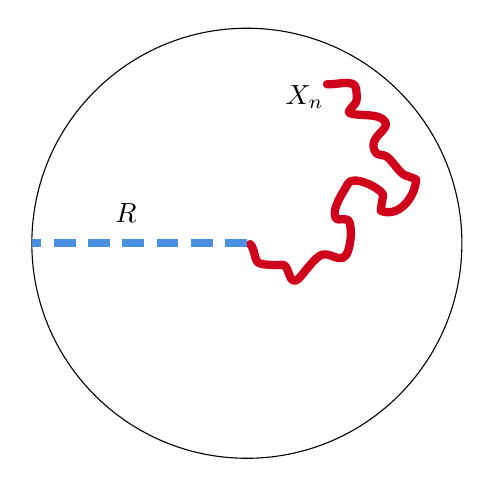
\begin{tikzpicture}[x=0.75pt,y=0.75pt,yscale=-1,xscale=1]
        %uncomment if require: \path (0,300); %set diagram left start at 0, and has height of 300

        %Shape: Circle [id:dp4944181906976386] 
        \draw   (219,150.6) .. controls (219,93.38) and (265.38,47) .. (322.6,47) .. controls (379.82,47) and (426.2,93.38) .. (426.2,150.6) .. controls (426.2,207.82) and (379.82,254.2) .. (322.6,254.2) .. controls (265.38,254.2) and (219,207.82) .. (219,150.6) -- cycle ;
        %Shape: Free Drawing [id:dp9400893360400799] 
        \draw  [color={rgb, 255:red, 208; green, 2; blue, 27 }  ,draw opacity=1 ][line width=3] [line join = round][line cap = round] (324.2,151) .. controls (326.46,153.26) and (326.14,158.63) .. (328.2,160) .. controls (330.41,161.48) and (340.03,160.95) .. (340.2,161) .. controls (343.25,161.83) and (342.65,171.19) .. (347.2,168) .. controls (348.78,166.89) and (355.57,156.6) .. (359.2,156) .. controls (364.43,155.13) and (369.91,163.22) .. (372.2,151) .. controls (372.81,147.72) and (373.01,144.23) .. (372.2,141) .. controls (371.14,136.75) and (366.39,140.97) .. (365.2,138) .. controls (363.45,133.62) and (369.58,125.24) .. (371.2,122) .. controls (373.46,117.49) and (385.96,123.41) .. (388.2,127) .. controls (388.41,127.34) and (386.87,134.88) .. (387.2,135) .. controls (394.01,137.55) and (399.51,132.39) .. (402.2,127) .. controls (403.29,124.83) and (403.86,122.4) .. (404.2,120) .. controls (404.26,119.56) and (399.97,118.26) .. (399.2,118) .. controls (396.19,117) and (393.25,111.44) .. (390.2,109) .. controls (387.85,107.12) and (385.81,109.23) .. (384.2,106) .. controls (380.81,99.22) and (391.86,95.99) .. (389.2,92) .. controls (386.34,87.7) and (377.73,89.58) .. (372.2,88) .. controls (370.77,87.59) and (373.15,85.05) .. (374.2,84) .. controls (375.83,82.37) and (375.79,80.69) .. (375.2,76) .. controls (374.62,71.32) and (365.9,74.36) .. (361.2,74) ;
        %Straight Lines [id:da614933324391667] 
        \draw [color={rgb, 255:red, 74; green, 144; blue, 226 }  ,draw opacity=1 ][line width=3]  [dash pattern={on 7.88pt off 4.5pt}]  (322.6,150.6) -- (219,150.6) ;

        % Text Node
        \draw (258,130.4) node [anchor=north west][inner sep=0.75pt]    {$R$};
        % Text Node
        \draw (340,73.4) node [anchor=north west][inner sep=0.75pt]    {$X_{n}$};


    \end{tikzpicture}
    \caption{Strategy for avoiding traps by not allowing the walk to move outside the ball of radius $R$}
\end{figure}
The strategy is to find an event such that $\P^X_{\epsilon}.(\text{event})\approx \sigma^{0}(x)$
We first define the following events:\\\\
$G_n=$ \{$X_n$ stays inside $B(0,R_n)$\}\\
$E_n=$\{no traps in $B(0,R_n)$\}\\
$F_n=$\{traps outside $B(0,R_n)$ by time $n$\}.\\\\
We get the probability of the given events as:
\begin{equation}
    \P(E_n)=e^{-cR_n^d}
\end{equation}
\begin{equation}
    \begin{aligned}
        \P(G_n) & =\P(\text{sup}_{0\leq k\leq n}|X_k|\leq R_n) \\
                & =\P(\tau_{B(0,R_n)}\geq n)                   \\
                & \geq e^{-cn/{R_n^2}}
    \end{aligned}
\end{equation}
and
\begin{equation}
    \begin{aligned}
        \P(F_n)\geq e^{-c\sqrt{n}}
    \end{aligned}
\end{equation}
Choose $R_n$, s.t.
$$
    c_1 R_n^d=c_2 n / R_n^2 \text{ i.e. } R_n=c_1 n^{1 / d+2}
$$
This shows that $P(G_n\cap E_n \cap F_n)$ is of the same order as $\sigma^\zero (n)$.
\end{document}